This chapter is adapted from the paper \citet{spohnSchedulingDirect2022}.
\section{Introduction}%
% \label{sec:introduction}
To increase the number of planets they can detect, direct imaging mission concepts, such as LUVOIR
\citep{TheLUVOIRTeam2019} and HabEx \citep{gaudiHabitableExoplanetObservatory2020}, are planning on using precursor information
from other exoplanet detection methods.  In their science and technology definition study, the HabEx
team identified extreme precision radial velocity (EPRV) as the most promising way to make precursor
observations  \citep{gaudiHabitableExoplanetObservatory2020}.  The study noted that one issue with orbital fits from radial velocity
(RV) measurements is that they can lose accuracy, or grow ``stale'', with time, but this effect has
not yet been fully quantified.  In this paper we aim to establish metrics that indicate when an RV
fit is no longer useful or is actively harmful in planning a direct imaging mission.

While fitting an orbit to an RV curve can be done in many ways, over the past 20 years the two
primary methods have been gradient descent and Bayesian Hierarchical modeling.  Gradient descent has
focused on using the Leveneberg-Marquardt (LM) algorithm \citep{Levenberg1943b, Marquardt1963b} and
the most common method for Bayesian modeling is the Markov Chain Monte Carlo (MCMC) method
\citep{Metropolis1953, Hastings1970}.  Currently, the most commonly used tools are based on
the MCMC method because it excels at fitting data with large uncertainties \citep{Wright2009b}.
Among the most popular radial velocity fitting software is \code{RadVel} \citep{fultonRadvelRadialVelocity2018}, which provides an
open-source and flexible implementation of this method.

The fits generated from RV signatures provide a lot of information that can be directly used for direct
imaging, such as the planet's period ($T$), eccentricity ($e$), and argument of
periastron ($\omega_p$).  However, the fits are unable to separate the planet's mass ($M_p$) and
inclination ($i$), instead fitting only the quantity $M_{p}\sin{i}$.  Because of this ambiguity,
making probabilistic statements on when a planet will be detectable relies on sampling from priors
on inclination or planet mass.

When an RV signature has negligible error, which is largely based on our understanding of stellar
variability, the orbital fit will give accurate estimates of times when a planet will be within a
direct imaging instrument's geometric constraints (i.e., falling between its inner and outer working
angles). An inaccurate fit's larger error bars, combined with the inherent RV ambiguity on mass and
inclination and the lack of photometric information (the exoplanet's radius, albedo, and phase
function), makes predicting when the exoplanet will be detectable very difficult.

Due to their low mass, the RV signatures of Earth-like exoplanets have amplitudes on the order of
tens of centimeters per second.  The current state-of-the-art RV measurements mostly have precisions
of around 1 m/s \citep{EPRV2020}, making them incapable of detecting Earth-like exoplanets.
The 1 m/s noise floor is due primarily to inter-night stellar variability, and higher precisions for single
night observations have been demonstrated by instruments such as ESPRESSO \citep{Pepe2021} and
MAROON-X \citep{Seifahrt2021}.  The EPRV initiative is targeting precision of a few
cm/s \citep{EPRV2020} in the next 10-15 years. 

In Section~\ref{sec:consistent_orbits} we look at four different methods of constructing
orbits that are consistent with the radial velocity curve, discuss desired performance, and
analyze the differences between the methods in Section~\ref{sec:construction_method_analysis}. To
quantify these differences we establish two modes of failure in Section~\ref{sec:fitting_failure},
and in Section~\ref{sec:failure_results} we simulate the full process of gathering RV data, fitting
the data with \code{RadVel}, constructing orbits using the four different methods, and propagating
the constructed orbits in time to see when they fail.

\section{Constructing consistent orbits}%
\label{sec:consistent_orbits}

The general procedure of constructing populations of orbits consistent with RV measurements is:
\begin{enumerate}
    \item Define a ground truth planet and a $1 \sigma$ error (representing both observatory and stellar
        noise) on RV measurements.
    \item Create synthetic RV observations of the ground truth planet with the assumed errors.
    \item Fit the synthetic RV observations with \code{RadVel}.
    \item Use \code{RadVel} outputs to sample many orbits consistent with the RV signal.
\end{enumerate}

\subsection{Synthetic RV data}%
\label{sec:synthetic_RV_data}

To create synthetic data we define the ground truth planet with a semi-major axis ($a$),
eccentricity ($e$), the planet's argument of periastron ($\omega_p$), inclination ($i$), planet mass
($M_p$), stellar mass ($M_s$), and true anomaly of the planet at the first moment of the simulated RV
campaign ($\nu_{p_0}$). We compute the planet's radius using the model from
\citet{savranskyExplorationDynamical2019} which is a modification of the \code{Forecaster} model \citep{chenProbabilisticForecastingMasses2016}
focused on exoplanets likely to be found via direct imaging.

The semi-amplitude $K$ is calculated using equation 2.27 from \citet{Perryman2018a}
\begin{equation}\label{eq:K}
    K = \left( \frac{2\pi G}{T}\right)^{1/3} \frac{M_p \sin(i)}{M_s^{2/3}} \frac{1}{\sqrt{1-e^2}} \,,
\end{equation}
where $T$ is the planet's orbital period, $G$ is the gravitational constant, and assuming the
approximation that $M_s+M_p \approx M_s$. 

All simulated RV curves in this work are based on the RV measurements of Gliese 849 b from the
HARPS database between 2004 and 2012 \citep{Mayor2003a}. To mimic the cadence of observations we
calculate the average number of RV observations per month, $\lambda $, from our dataset. With
$\lambda $ as the expected separation in time of observations we sample a Poisson distribution for every
month between the start of 2000 and the start of 2010 to get a discrete number of observations in
each month. Within each month the observation times are distributed according to a random uniform
distribution.

At those synthetic RV observation times we calculate the true anomaly of the star, $\nu_s$, with
Newton-Raphson root-finding \citep{Murray2000}.  The radial velocity, neglecting barycenter motion, can then be found
as \citep{Perryman2018a}
\begin{equation}
    v_s = K \left(e \cos(\omega_s) + \cos(\nu_s + \omega_s)\right) \,,
\end{equation}
where $\omega_s$ is the star's argument of periastron, equal to $\omega_{p}+180\degree$.  This
process is repeated at every observation time to create the ``true'' radial velocity signature of
the planet over a set range of time.  To simulate noise on the observations, we draw the
``observed'' RV value of each observation from a normal distribution with the mean at the true
radial velocity value and the $1 \sigma$ error equal to the defined $1 \sigma $ error which
represents observatory and stellar noise. Note that there are many different potential sources of
error on RV measurements \citep[see, e.g.,~][]{Fischer2016a}, which we are combining into a single
$1 \sigma $ value to match the assumed inputs to \code{RadVel}, which are a time series of observed
radial velocities and their $1 \sigma $ values. To be clear, the defined 1 $\sigma $ error
is not based on a specific instrument or noise source, but rather represents a
simplified parameter that can be varied in order to test the effects of
different RV precisions.


\subsection{Fitting the RV curve}%
\label{sec:rvfit}
We use \code{RadVel} \citep{fultonRadvelRadialVelocity2018} to create an
orbital fit from our noisy, synthetic data. The fitting basis used is the
\code{RadVel} standard for fitting: $T$, $T_c$ (time of conjunction),
$\sqrt{e}\cos{\omega_s}$, $\sqrt{e}\sin{\omega_s}$, $K$.  Gaussian priors are
assigned to $T_c$ and period $T$. To simulate imperfect information about the
planet we offset the Gaussian priors used by \code{RadVel} for $T$ and $T_c$.
This is done by sampling a normal distribution centered on the true mean with a
1$\sigma$ error of 10\% of $T$. This prior assumes that $T$ and $T_c$ can be
determined in part based on analysis of the RV time series before using
\code{RadVel}. A Nelder-Mead \citep{Nelder1965,Gao2010a} optimization is then
run on the posterior to refine it. Then the fitting is done using the
\code{RadVel} implementation of the MCMC package \code{emcee} \citep{emcee}.
The MCMC analysis provides the fitting basis parameters and the likelihood
associated with each step of the Markov Chain.

\subsection{Transforming Fitting Basis to Keplerian Elements}
To simulate imaging observations we need to be able to propagate in time and find the separation and
brightness at any time step. Because of this we must calculate the Keplerian orbital parameters
that were defined to create the synthetic RV data shown in Section~\ref{sec:synthetic_RV_data} 
The eccentricity $e$ is given by 
\begin{equation}
     e = \left( \sqrt{e} \cos(\omega_s) \right)^2 + \left( \sqrt{e} \sin(\omega_s) \right)^2
\end{equation}
and the argument of periastron is given by
\begin{equation}
    \omega_s = \arctan\left(\frac{\sqrt{e} \sin(\omega_s)}{\sqrt{e} \cos(\omega_s)}\right) \,,
\end{equation}
with $\omega_p = \omega _s + 180\degree$. The time of periastron requires
several more intermediate calculations.  Using the geometry shown in Figure 1
of \citet{fultonRadvelRadialVelocity2018} we can express the true anomaly of
the planet, $\nu_p$, at the time of conjunction as
\begin{equation}
    \nu_p = 90\degree - \omega_s \,.
\end{equation}
With this we can find the eccentric anomaly of the planet at the time of conjunction as
\begin{equation}%
    \label{eq:ecc_anom}
    \tan \left( \frac{E}{2}\right) = \sqrt{\frac{1-e}{1+e}} \tan \left(\frac{\nu}{2}\right)
\end{equation}
and solve for the mean anomaly at that time with Kepler's equation
\begin{equation}%
    \label{eq:mean_anom}
    M = E - e \sin{E} \,.
\end{equation}

We find the time of periastron passage as
\begin{equation}
    T_p = T_c - \frac{M}{n} = T_c - \frac{M T}{2\pi}
\end{equation}
where $n$ represents the orbital mean motion.
The semi-major axis ($a$) is a function of the period and gravitational parameter $\mu=G M_s$ (again using
the approximation $M_p + M_s \approx M_s$)
\begin{equation}
    a = {\left( \mu {\left(\frac{ T}{2\pi}\right)}^2 \right)}^{1/3} \,.
\end{equation}
Using equation~\ref{eq:K} we can calculate the quantity $M_p\sin{i}$ based on the fit values of $K$,
$e$, and $T$. However, the $M_p \sin{i}$ quantity cannot be separated into $M_p$ and $i$ without
making further assumptions.

\subsection{Methods of constructing consistent orbits}\label{sec:orbit_methods}
Since the end goal of this work is to analyze how well RV data can be utilized for planning direct imaging observations we
need a metric based on an RV signal that quantifies when a planet will be detectable for a direct
imaging instrument.  Our approach is similar to the calculation of completeness for planetary
populations \citep{brownObscurationalCompleteness2004,
brownSingleVisitPhotometric2005, brownNewCompletenessMethods2010,garrettAnalyticalFormulation2016}.
This approach relies on constructing a
large set of orbits that a planet could be on and describing the probability of making a detection
as 
\begin{equation}\label{eq:prob_det}
    P_{\textrm{det}}(t) = \frac{\textrm{Number of orbits detectable at time $t$}}{\textrm{Number of
    constructed orbits}}
.\end{equation}
Unlike Brown, we are basing the orbits on prior information from the RV curve gathered from the 
\code{RadVel} fit, rather than drawing from assumed distributions of parameters describing some population
of planets.

Currently, there is no single universally agreed upon method to create the large set of orbits
necessary for Equation~\ref{eq:prob_det} to give reliable results. To fill that gap we have analyzed
four different ways of using \code{RadVel}'s outputs for that purpose. Ideally, the set of orbits
generated will lead to accurate predictions of when the planet is detectable while avoiding
predictions that the planet will be detectable when it isn't.

Each of the methods, described below, begins by generating values for $a$, $e$, $\omega_p$, $T_p$, and $M_p \sin
i$ and then sampling a prior distribution on $i$ to separate the planet mass and inclination.
\subsubsection{Maximum Likelihood}
In this method we take the fitting basis parameters ($T$, $T_c$, $\sqrt{e} \cos{\omega_s}$, $\sqrt{e}
\sin{\omega_s}$, $K$, as described in Section \ref{sec:rvfit}) from the MCMC step with the highest likelihood.
This means that the only source of variation in the constructed orbit population comes from sampling
the prior on $i$ to split up the $M_p \sin i$ quantity.

\subsubsection{Maximum Kernel Density Estimate (KDE)}
The kernel density estimate of the fitting basis is found using Scott's method \citep{Scott1992}.
We then use the Broyden–Fletcher–Goldfarb–Shanno (BFGS) minimization routine
\citep{Nocedal2006}, as implemented in SciPy
\citep{virtanenSciPyFundamental2020}, to find the parameter set that maximizes the kernel density
estimate. Like the maximum likelihood method above, this creates a single set of parameters from the
fitting basis and all variations are in $i$ and $M_p$ due to sampling the inclination prior.

\subsubsection{Credible Interval}
\code{RadVel} defines a ``Credible interval'' for a parameter as the median and standard deviation of the
fitting basis parameters for every step taken during MCMC analysis. 
This method takes that same approach, calculating the median and standard deviation for each
fitting basis parameter based on every step of the MCMC analysis.
Then to create orbits we sample each fitting basis parameter independently, treating each as normally distributed based on their median and standard deviation. Unlike the previous two methods of
generating orbits, this one has variation in all orbital parameters, as well as inclination and planet mass.

\subsubsection{Multivariate Gaussian}
To get a distribution of high likelihood orbital parameters, the MCMC steps are sorted by likelihood
and the fitting basis parameters of the top 1000 are selected, from the hundreds of
thousands of MCMC steps, to compute a covariance matrix. We found that 1000 steps were enough to
identify the high likelihood regions while keeping computation times low. Using the
covariance matrix of MCMC parameters we can construct new sets of fitting basis parameters by
sampling a multivariate Gaussian. Sampling in this way lets us generate many more high
likelihood parameter sets than the chains alone provide without disregarding correlations between
the fitting basis parameters, most notably the relationship between $T$ and $T_c$. Like the credible
interval method above, this results in many different combinations of orbital parameters.

\subsection{Inclination Sampling}%
\label{subsub:inclination_sampling}
For each parameter set created by the methods described above, the inclination and mass ambiguity is
explored by sampling from the inclination distribution. Using the isotropic orbit orientation
assumption described in \citet{Savransky2011a} the inclination is distributed sinusoidally between
$0$ and $\pi$ radians, such that $i \sim \cos^{-1}\left(U\right)$ where $U$ represents a uniformly
distributed random value between -1 and 1. Further, we can impose certain constraints onto the mass
that narrow the inclination space. As $\sin{i}$ goes to 0, the planet's mass goes to infinity so we
impose restrictions on what inclinations are possible. Depending on a stellar object's chemical
composition it will begin hydrogen burning when its mass is above $\sim 0.07-0.09 M_{\odot}$
\citep{Perryman2018a}, at which point the object is no longer classified as a planet.  We use
the median point in that range to define a critical inclination
\begin{equation}
    i_{crit} = \arcsin\left(\frac{M_p \sin{i}}{0.08 M_{\odot}}\right) \,.
\end{equation}
To find a distribution of potential inclinations we sample from the prior sinusoidal distribution,
limited by $i_{crit}$, and solve for the corresponding $M_p$ value for each
inclination. The planet's radius is calculated using the same method from
Section~\ref{sec:synthetic_RV_data}.

\subsection{Propagation in time}
The constructed orbits now have all the information necessary to simulate their motion.  Using the time of
periastron $T_p$ we can find the mean anomaly at each desired time step $t$
\begin{equation}
    M(t) = n (t - T_p)
\end{equation}
which is used as an intermediate step for the desired direct imaging parameters, the difference in
brightness magnitude between the planet and star ($\Delta\mathrm{mag}$) and the angular separation
between the planet and star ($\alpha$).  To find those we first calculate the planet's true anomaly,
$\nu_p$ from its mean anomaly using Equations~\ref{eq:ecc_anom}--\ref{eq:mean_anom}, again via Newton-Raphson. The orbital radius $r$ is given using the
equation
\begin{equation}%
    \label{eq:r}
    r = \frac{a \left( 1 -e^2 \right) }{1 + e \cos \nu_p } \;
.\end{equation}
Then we find the projected separation
\begin{equation}
    s = \frac{r}{4} \sqrt{4 \cos{2i} + 4 \cos{2\theta} - 2\cos( {2i-2\theta} ) - 2\cos({2i+2\theta}) + 12} \,.
\end{equation}
where $\theta = \nu_p + \omega_p $ is the argument of latitude of the planet.
From this and the distance to the star $d$, we calculate the angular separation
\begin{equation}%
    \label{eq:alpha}
    \alpha = \tan^{-1}\left( \frac{s}{d} \right)
.\end{equation}
The phase angle $\beta$ is calculated as
\begin{equation}%
    \label{eq:beta}
    \beta = \arccos( {-\sin{i}\sin{\theta}} )
\end{equation}
under the assumption that $d \gg r$ and that the observer is looking down on the orbital plane, as described in \citet{savranskyExplorationDynamical2019}.
The photometry calculations assume Lambertian scattering and use Lambert's phase function
\begin{equation}
    \Phi(\beta) = \frac{1}{\pi} \left( \sin\beta + (\pi-\beta) \cos\beta\right) \,.
\end{equation}
We find the flux ratio $F_R$, or the ratio of the planet's flux $F_p$ over the star's flux $F_s$,
as
\begin{equation}
    F_R = \frac{F_p}{F_s} = p\Phi(\beta)\left(\frac{R_p}{r}\right)^2 \,.
\end{equation}
For the purpose of these simulations all planets are assigned the Earth's geometric albedo $p$ of
$0.367$ as in \citet{Seidelmann2006}.
The difference in magnitude between star and planet, $\Delta\mathrm{mag}$, is
\begin{equation}
    \Delta\mathrm{mag} = -2.5\log_{10}F_R \,.
\end{equation}

\subsection{Orbit detectability}
With $\alpha$ and $\Delta\mathrm{mag}$ we can compare the visibility for each
planet against the constraints of the observatory to calculate visibility. A detectable planet will
meet the criteria
\begin{align}
    \text{IWA} < \alpha < \text{OWA}\label{eq:alpha_constraint}\\
    \Delta\mathrm{mag} < \Delta\mathrm{mag}_0\label{eq:dMag_constraint}
\end{align}
where IWA is the observatory's inner working angle, OWA is the outer working angle, and
$\Delta\mathrm{mag}_0$ is the observatory's limiting difference in brightness \citep[effectively equivalent to the instrument contrast capability---for further discussion see][]{Brown2005d}. Using these
constraints, the method of propagation, and equation~\ref{eq:prob_det} we can calculate the
probability of detection as a function of time.
\section{Construction method analysis}%
\label{sec:construction_method_analysis}
\begin{figure}[htpb]
    \centering
    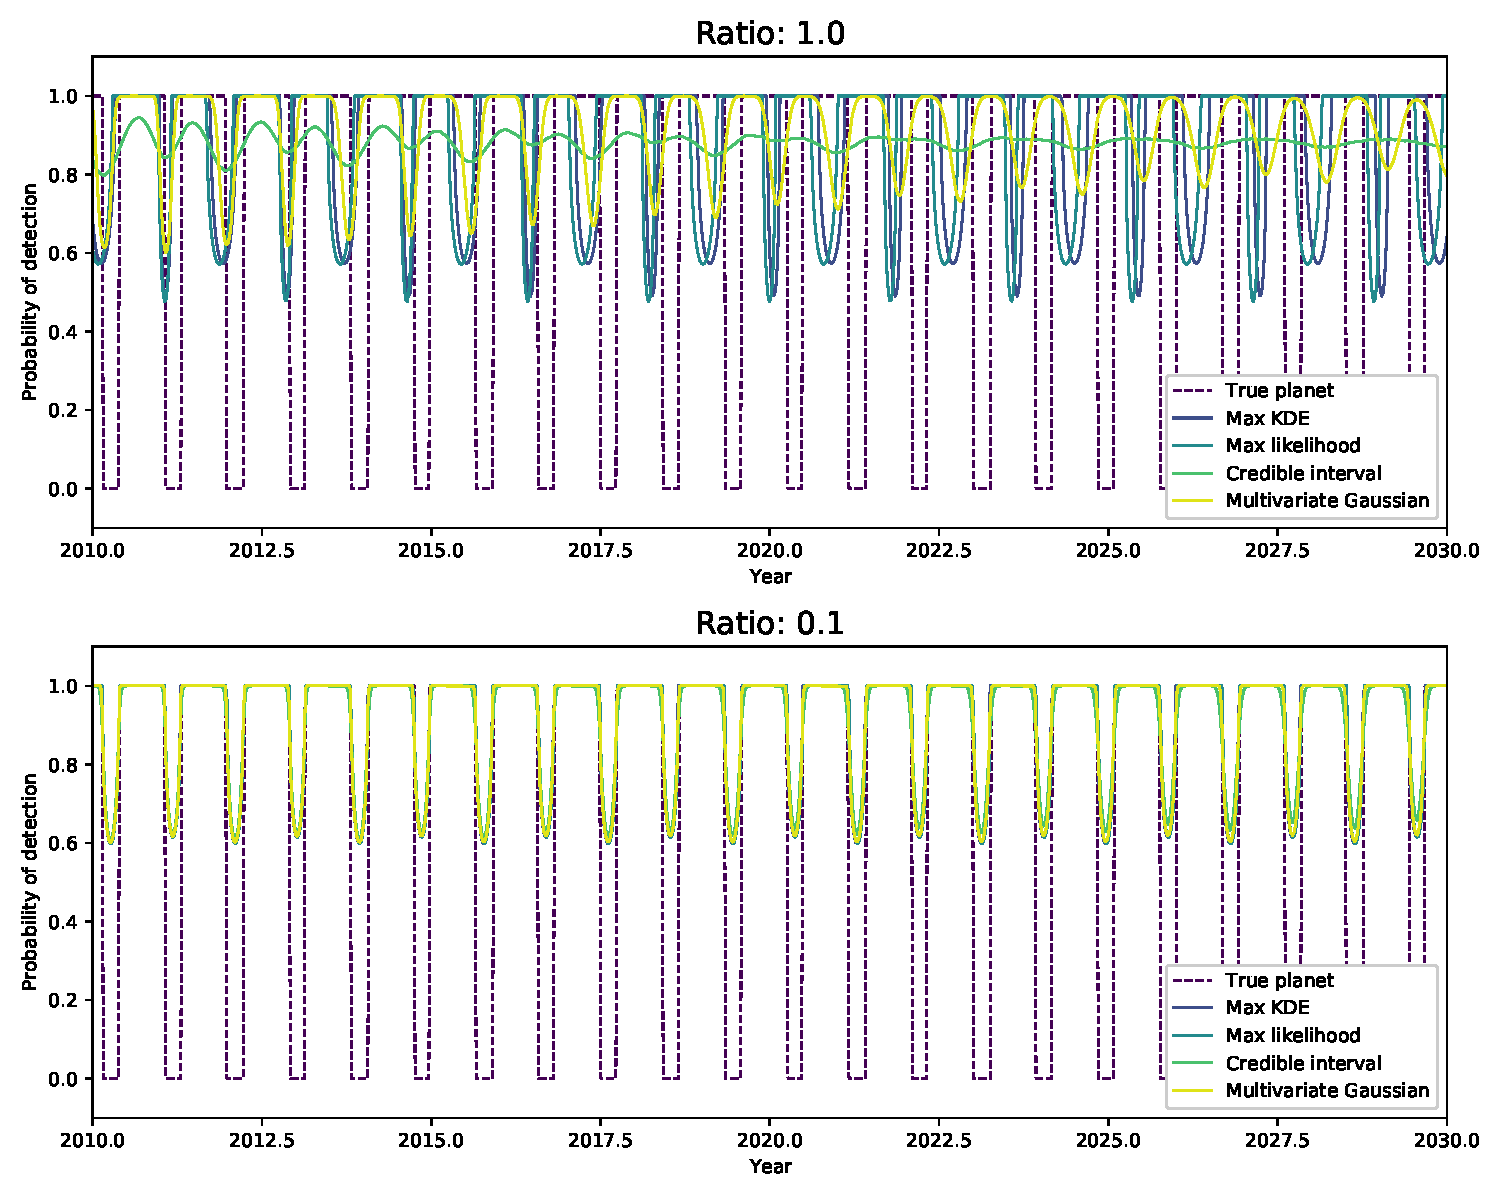
\includegraphics[width=\linewidth]{ch1/figures/prob_det_new.pdf}
    \caption{Comparison of how the four different orbit construction methods (max KDE, max
    likelihood, credible interval, and multivariate Gaussian) perform at calculating the
    probability of detection at two different ratios of RV error to RV semi-amplitude. The ``True
    planet'' line has a value of 1 when the defined planet is detectable by a HabEx-like instrument, and a value of zero when it is not.}%
    \label{fig:prob_det_comparison}
    %Note: the reason that 1.0 max L plot is so varied is because its e is 0.52
\end{figure}
\begin{figure}[hpt]
    \centering
    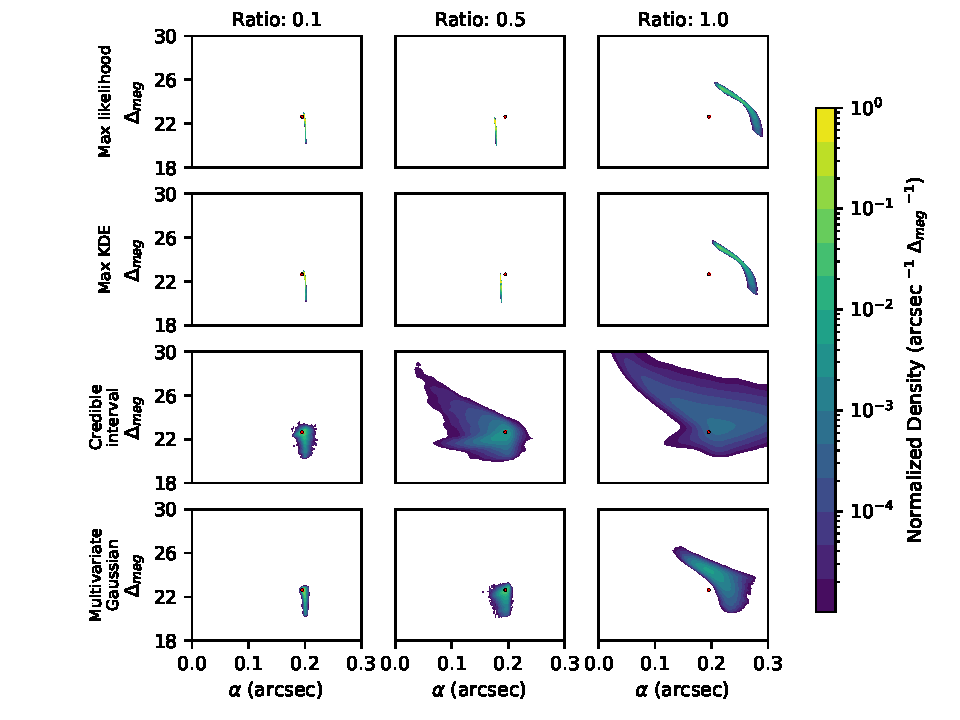
\includegraphics[width=\linewidth]{ch1/figures/construction_method_vs_error_100.pdf}
    \caption{Distributions in $\alpha $ vs $\Delta\mathrm{mag}$ space for the different orbit construction
    techniques at the time of fitting. The point represents the true planet's location. The planet
    has $a$ of 2 AU, $e$ of 0, $i$ of 100\degree, $R_p$ of $3.48 R_{\bigoplus}$, geometric
    albedo of 0.367, and is around a Sun-like star at a distance of 10 parsecs. Each column uses the
    same output from \code{RadVel} with a set ratio of RV error to RV semi-amplitude and assumes 10
    years of radial velocity measurements.}%
    \label{fig:construction_method_pdfs}
\end{figure}
\begin{figure}[htpb]
    \centering
    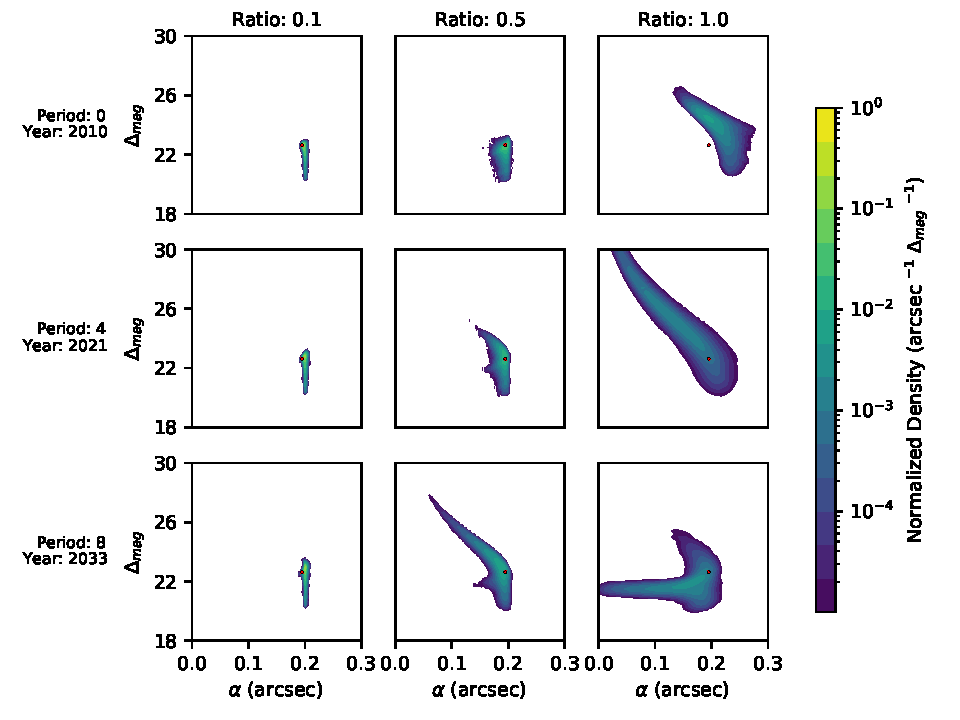
\includegraphics[width=\linewidth]{ch1/figures/dispersion_in_time_i100.pdf}
    \caption{Temporal evolution of orbits constructed with the multivariate Gaussian method shown in
    Figure~\ref{fig:construction_method_pdfs}.}%
    \label{fig:dispersion_in_time}
\end{figure}
We tested the different methods of creating consistent orbits laid out in
Section~\ref{sec:orbit_methods} using a super-Earth on an edge-on orbit, as shown in
Figure~\ref{fig:prob_det_comparison}. We see that there is not much difference between the
performance of the different construction methods when the ratio of error to semi-amplitude is low.
However, when the ratio is high the different construction methods diverge significantly in their
predictions of planet detectability.

The methods that create distributions of the fitting basis parameters (credible interval and
multivariate Gaussian) have their features decay in time.  This is especially clear for the credible
interval curve, which begins with a low amplitude wave that peaks while the true planet is visible
and decays to a nearly constant value after 10 years. That decay represents the predictive power of
the consistent orbits decreasing as time goes by. The multivariate Gaussian curve decays, but to a
lesser extent.  It no longer reaches a probability of 1 by the end of the 20 years, but still
has significant oscillations.  The two methods that rely on a single set of fitting basis parameters
(max likelihood and max KDE) never decay, but this leads to many times when the true planet is not
detectable while the predicted probability of detection is unity.

Differences in this decay are further explored in Figure~\ref{fig:construction_method_pdfs} which
shows the joint density of the angular separation-$\Delta _{\textrm{mag}}$ phase space for the
various construction methods for a planet with a close to edge-on orbit, ($i=100\degree$ ). Note
that this figure represents a single scenario of orbital parameters and will vary greatly depending
on the orbital parameters and the quality of the RV measurement data. The max likelihood and max KDE
methods produce very clustered orbits. In this scenario however (and in most scenarios as we show in
Section~\ref{sec:failure_results}), none of the distributions created by either max likelihood or
max KDE methods include the true planet. That will lead them to make inaccurate predictions for
detectability. The large spread shown by those two methods for the ratio of one is due to the max
KDE and highest likelihood fitting basis sets having high eccentricity which, combined with the
inclination sampling, produced a lot of variability in the separation-$\Delta \mathrm{mag}$ space.
The orbits constructed with the credible interval method show the largest overall variance. For
small error to semi-amplitude ratios, the orbits constructed with the credible interval method
cluster around the true planet's location, but the distribution rapidly grows in size as the ratio
increases.  
In this case the ``true'' planet remains in the high
density regions of the orbits constructed with the credible interval method. However, for ``true''
planets with higher inclinations this would not be the case because the prior on inclination
produces more edge-on orbits.  While the plots in Figure~\ref{fig:construction_method_pdfs} are for
a single, specific set of values for the planet and orbital parameters and stellar distance, they
can be easily scaled for any variation of the parameters.  The angular separation, as given in
Equation~\ref{eq:alpha}, scales nearly linearly (in the small-angle approximation) with both
semi-major axis (directly) and stellar distance (inversely). For changes in semi-major axis,
$\Delta\mathrm{mag}$ scales as $\Delta\mathrm{mag} - 5\log_{10}\left(\frac{a}{a_0}\right)$ where
$\frac{a}{a_0}$ is the ratio of the new to original semi-major axis. Changes in geometric albedo or
planet radius will similarly additively change the $\Delta\mathrm{mag}$ while not affecting the
angular separation.

In the scenario shown in Figure~\ref{fig:construction_method_pdfs}, the multivariate Gaussian orbit
construction method maintains a tighter density than the credible interval method while still
including the true planet for ratios 0.1 and 0.5, which the two max methods do not, but does not
include the true planet for a ratio of 1. Similar to the credible interval method, for large
inclinations the true planet will drift further away from the high density regions of the
distributions.

Figure~\ref{fig:dispersion_in_time} further explores the information decay in time, showing how the
orbits disperse at three different times.  In this case we use the multivariate Gaussian method, but
the plot has similar features for the credible interval method.  Each time corresponds to an integer
orbital period so that the true planet is at the same location along its orbit. For all three ratios
we see that the distribution disperses significantly in time.  Unsurprisingly, the spread in the
distribution is proportional to the assumed error ratio, with the lowest ratio showing little change
after even 8 full orbital periods (in this case 23 years). In every case except one the true planet
remains within a region where the orbit distribution has a normalized density above $10^{-5}$, but
clearly the predictive power of the orbits constructed from noisy RV fits decreases in time.

\section{Fitting failure}%
\label{sec:fitting_failure}

Having established methodologies for sampling orbits consistent with RV data, we can now evaluate
how well our different construction methods perform in scheduling direct imaging observations. A
successful orbit fit will show a high probability of detection when the true planet is visible, dip
when the true planet is not visible, and continue to do so consistently over many orbital periods.
We have identified two primary types of fitting failure, which we call intermittent failure and
dispersion failure. Intermittent failure occurs when an orbital fit indicates a high probability of
an observation yielding a detection at a time when the true planet is not detectable. Dispersion
failure occurs when the probability of detection curve flattens, at which point the orbital fit
gives little information on when an observation should be scheduled.

\subsection{Intermittent failure}%
\label{sub:intermittent_failure}
\begin{figure}[htpb]
    \centering
    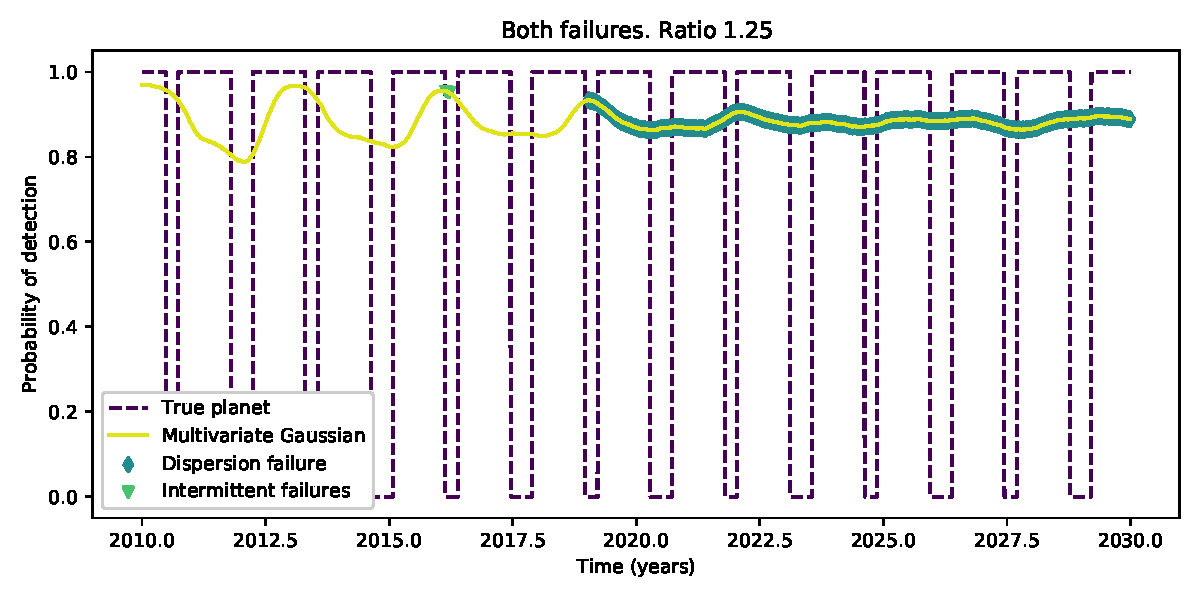
\includegraphics[width=\linewidth]{ch1/figures/prob_det_vs_time_both_failure.pdf}
    \caption{Probability of detection curve demonstrating both kinds of failure. The green triangles represent steps
    when all conditions for intermittent failures are met. The end of the curve, highlighted,
    represents the point in time when dispersion failure has occurred. This is a somewhat
    extreme example as it is unlikely that a planet with an error to semi-amplitude ratio of 1.25
    would be considered for observation.}%
    \label{fig:figures/both_failures}
\end{figure}
The point of intermittent failure is to identify times when a mission scheduler would plan an
observation with confidence even though it would lead to a null detection.
Figure~\ref{fig:figures/both_failures} shows a peak marked as an intermittent failure because it is a
high and relatively stable probability of detection at a time when the true planet is not visible.
Observing at that time would be seen as a good idea, but lead to a failed detection of a planet that
is detectable for the majority of the mission. Intermittent failure occurs when all of
the following conditions are met:
\begin{enumerate}
    \item The true planet is not detectable;
    \item The estimated probability of detection is in the top 90\% of the local probability of
        detection values;
    \item The probability of detection is changing by less than 0.0001 per day; and
    \item The previous three conditions hold for 1 day.
\end{enumerate}
Note that the numerical values given in the conditions have been used for this analysis and were
determined heuristically based on what we assume someone scheduling a direct imaging mission would
see as satisfactory information that an observation will result in a detection. For a specific
mission the values should be optimized based on the goals and constraints of that mission.

The first condition exists to focus on times when a scheduled observation would result in a failed
detection. Note that this condition makes it so that if a planet is always detectable, such as
face-on orbits, no orbital fit can produce an intermittent failure.  The second condition exists
because the orbit construction methods, primarily those that have multiple fitting basis parameters
such as credible interval and multivariate Gaussian, will produce probability of detection curves
that don't always reach unity, and additionally the peaks decay in time (as shown in
Figure~\ref{fig:prob_det_comparison}). By describing it in terms of a local range of values we avoid
restricting our observations to an absolute threshold that may not be met even though the detection
curve is peaking when the true planet is detectable. The second condition can be expressed as
$P_{\textrm{det}} > \left(0.9 \left(  \textrm{local max} - \textrm{local min}\right) + \textrm{local
min}\right)$.  The third condition exists because there are many times when the first two conditions
are met while a large percentage of orbits consistent with the RV observations are entering
or exiting the direct imaging instrument constraints, causing the probability of detection curve
to change rapidly. We assume that a mission scheduler would avoid such times, preferring to
observe when the number of orbits detectable is stable.
To demonstrate the relevance, without the third condition the curves in Figure~\ref{fig:prob_det_comparison}'s
bottom plot would be considered in intermittent failure immediately before the true planet becomes
detectable and immediately after it is not detectable, even though it is clearly better to observe
in the long time period when the probability of detection is stable at unity, not right before or
after that time period. The last condition exists to rule out the times when the first three
conditions are met for a time shorter than an observation would be scheduled for, which should be
tuned based on the required integration time of an observation.

To determine the local maxima required for the second condition we break the probability of
detection curve into different sections based on the extremum. The
first section begins at the initial time if the first extremum is a local maximum, or begins at the
first minimum if the first extremum is a local minimum. Then each subsequent section begins at each
subsequent minimum. The last section ends at the last minimum if the last extremum is a local
minimum, and the last point if the last extremum is a local maximum. Within each section, the local
probability of detection maximum is the greatest probability of detection in the section. To make
the peak finding robust we require the maxima to be at least 0.05 above the greater of the two
nearest minima, and the converse requirement was used for determining the minima. Lowering the 0.05
number will make the metric describe flatter regions, which better describes complete dispersion.
However, there is little reason to lower it because in situations when the probability of detection
is varying by less than 0.05 the orbits are so dispersed that the orbital fit is not providing
useful information about when to schedule observations, which is captured by the second failure
metric called dispersion failure.

\subsection{Dispersion failure}% 
\label{sub:dispersion_failure} 

Dispersion failure occurs when the probability of detection curve flattens to the point where a full
orbital period passes without any extrema, for the probability of detection curve as defined above.
Figure~\ref{fig:figures/both_failures} shows dispersion failure occurring 9 years after the
collection of the data used for the orbital fit.  If the constructed orbits have a wide range of
orbital parameters the probability of detection curve will show little change from the beginning,
such as the ``Credible interval'' curve for a ratio of 1 in Figure~\ref{fig:prob_det_comparison}.
The primary cause of dispersion is from many constructed orbits having different periods, making the
initial cluster of orbits disperse quickly.  Past the point of dispersion failure, there is no reason
for a mission scheduler to favor one point in time for observation over another, based on the
information from an RV fit.

\section{Failure results}%
\label{sec:failure_results}
\begin{figure}[htpb]
    \centering
    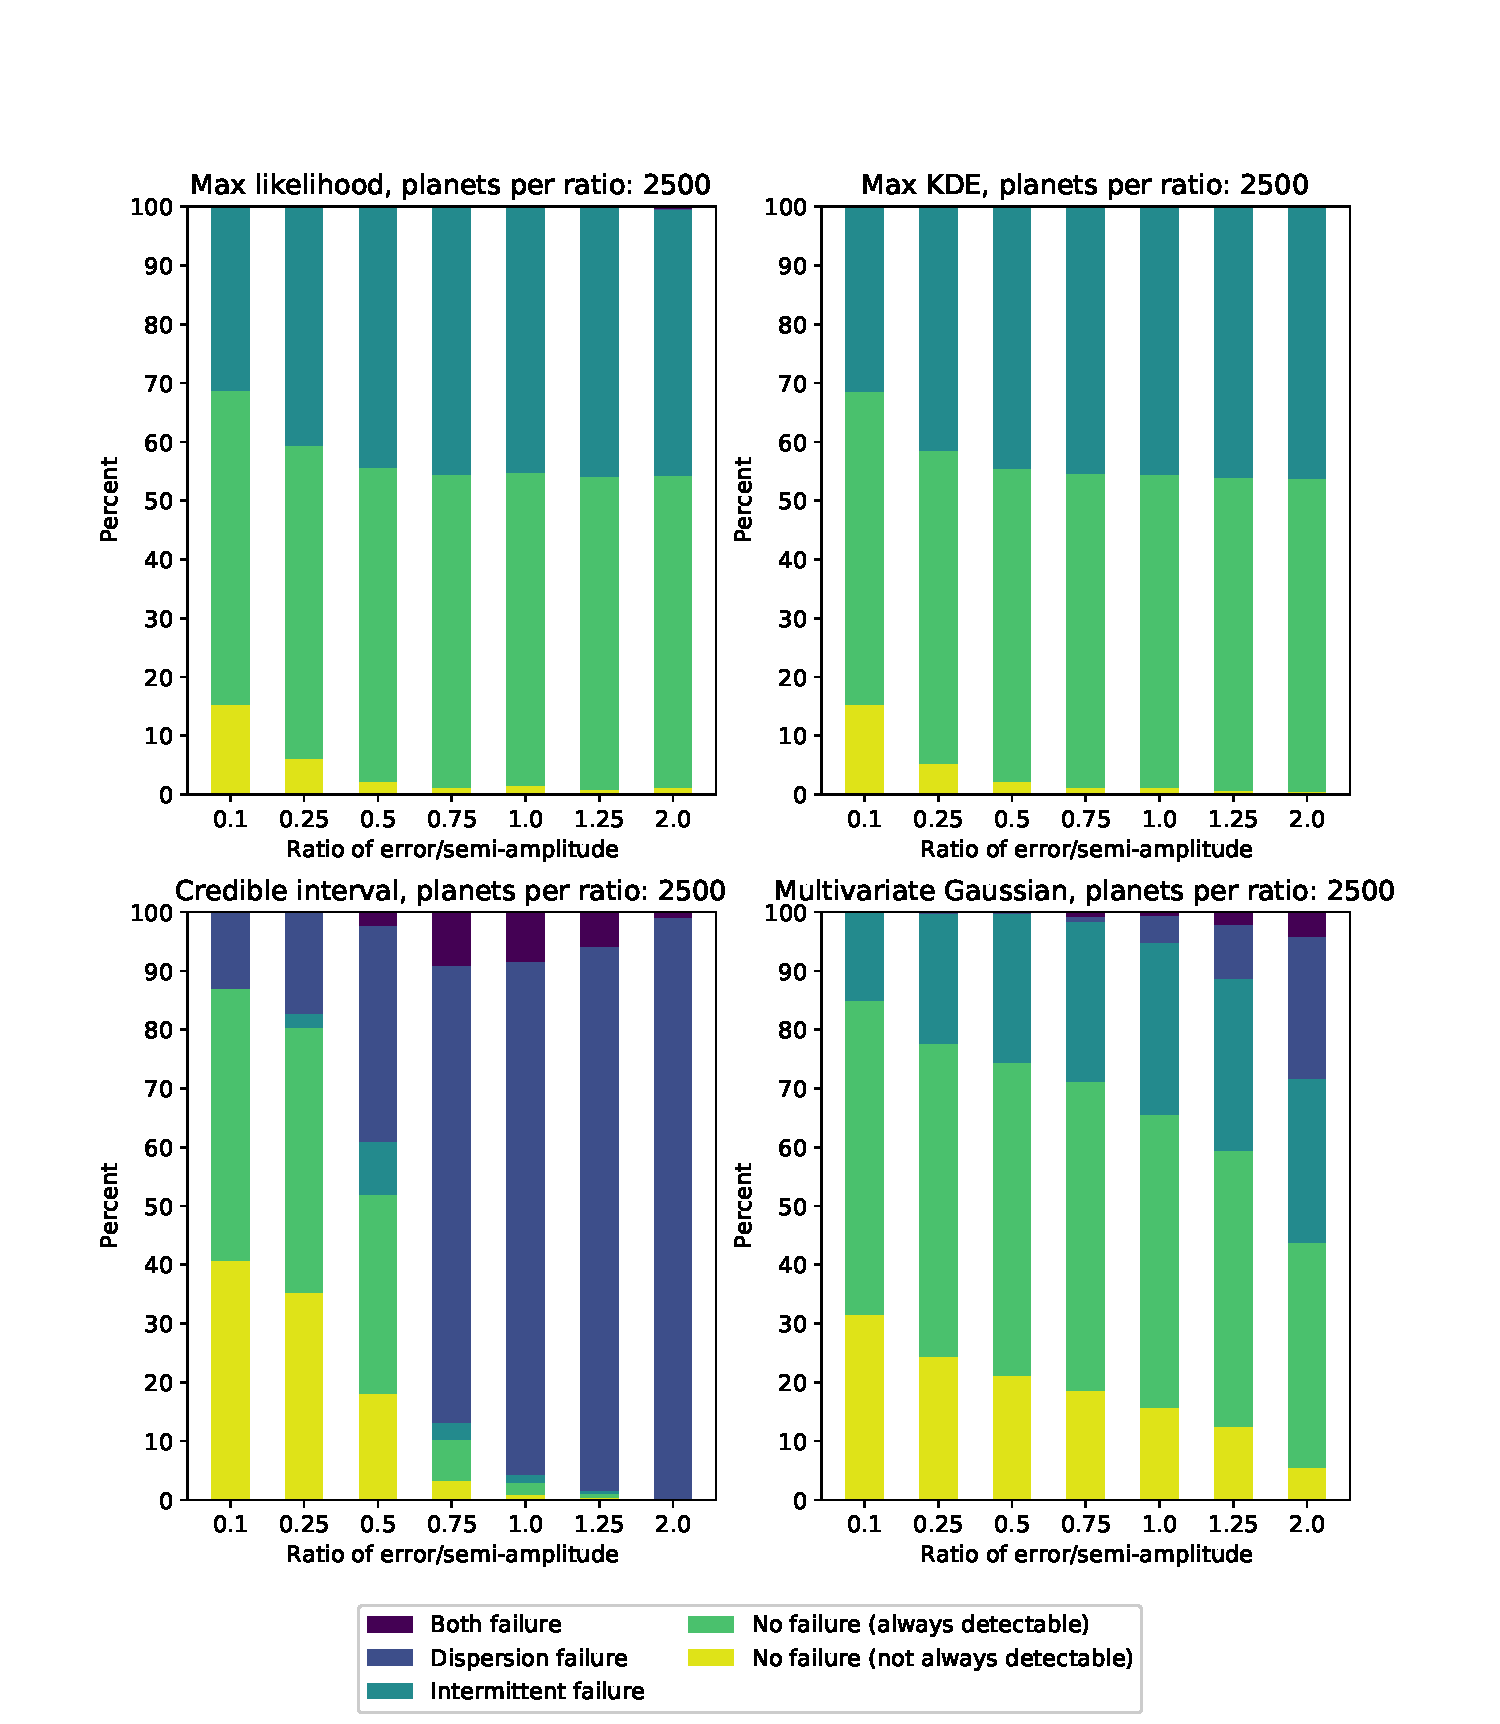
\includegraphics[width=\linewidth]{ch1/figures/construction_method_bars_including_always_detectable.pdf}
    \caption{Failure mode statistics for the four different construction methods for different
        ratios of RV error to signal semi-amplitude. We see that the failure percentage increases at
        different rates for each construction method as the ratio of error to semi-amplitude
        increases. Max likelihood and max KDE perform poorly for all ratios tested.  Credible
        interval performs the best for very low ratios and multivariate Gaussian significantly
        outperforms credible interval for ratios of 0.5 or greater. Note that while max likelihood
        and max KDE appear to perform well, this is only the case when the planet is always detectable
        which makes it a trivial result.}%
    \label{fig:con_method_bar_comparison}
\end{figure}
\begin{figure}[htpb]
    \centering
    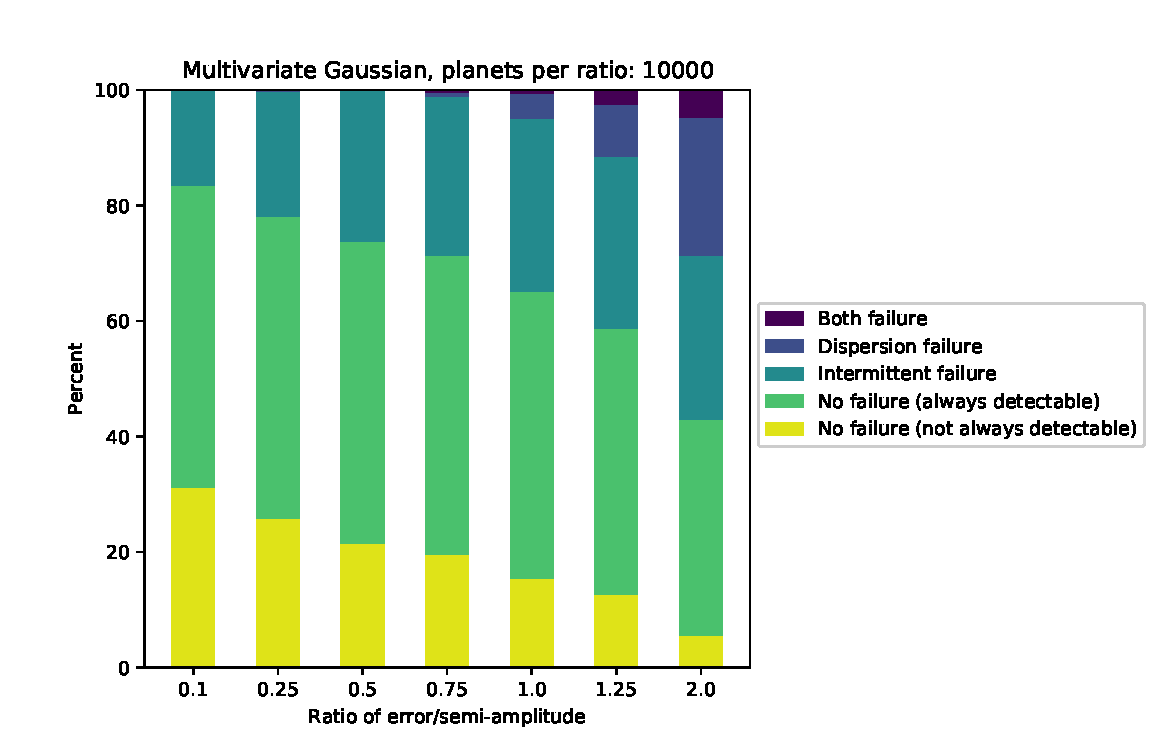
\includegraphics[width=\linewidth]{ch1/figures/total_bar_plot.pdf} 
    \caption{Results for multivariate Gaussian construction method with 10000 planets generated to
        test how representative the smaller sample of Figure~\ref{fig:con_method_bar_comparison} is.
        In all cases, the percentages match to better than 1.38\% and most below 0.35\%, lending confidence to the smaller
        sample size used in Figure~\ref{fig:con_method_bar_comparison}.}%
    \label{fig:bar_plot}
\end{figure}
\begin{figure}[htpb]
    \centering
    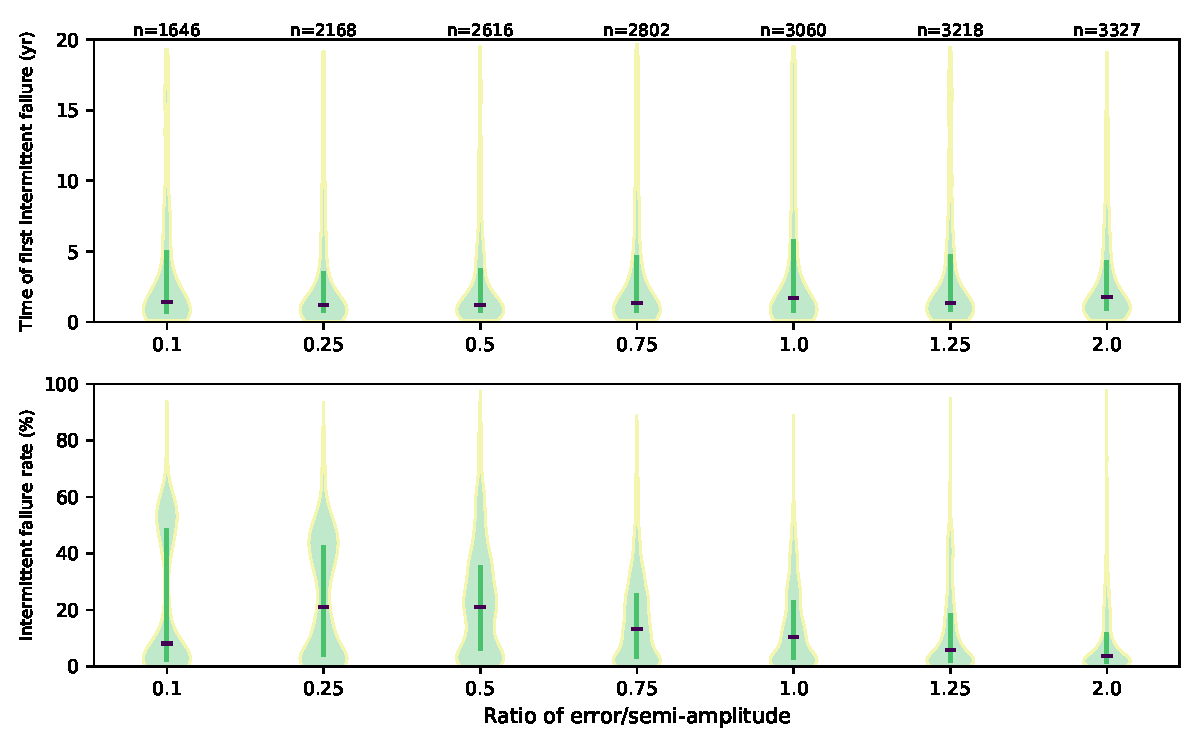
\includegraphics[width=\linewidth]{ch1/figures/violin_plots.pdf}
    \caption{Violin plots showing the variation of intermittent failure based on the ratio of RV
        error to RV semi-amplitude for the multivariate Gaussian method. Each violin shows the
        median (the horizontal black bar), the quartiles (the vertical green bars), and the kernel
        density estimate (the green curve to the left and right). The number of data points used for
        each ratio is labeled above the upper plot. We see that the distribution of the time of the
        first intermittent failure is weighted heavily near the start of the simulation with long
        tails for all ratios.  The intermittent failure rate is the number of intermittent failures
        divided by the number of times when the planet is not detectable. It is more variable, with
        low ratios having their distributions skewed to higher failure rates.  This is due to the
        dense clustering of orbits for low ratios, causing large failure rates when there is a
        period offset from the true planet.}%
    \label{fig:violin}
\end{figure}

To quantify how the ratio of RV error to RV semi-amplitude affects the scheduling of direct
imaging observations we fixed the semi-amplitude at 1 m/s and varied the RV error. We tested 
1$\sigma$ errors on RV measurements of 0.1, 0.25, 0.5, 0.75, 1, 1.25, and 2 m/s.  To generate true
planets we fixed $e$ at 0, $\omega$ at 0, $p$ at 0.367, mean anomaly at the initial time of RV
observation at 0, the star's mass at 1 solar mass, and set the star's distance to 10 parsecs. To
introduce variability we sampled 250 inclinations between 90 and 170 degrees based on a sinusoidal
distribution and generated 2500 planets by applying those inclinations to 10 linearly spaced $a$
values between 1 and 2 AU. To fix the semi-amplitude $K$ at 1 m/s we use equation~\ref{eq:K} to
calculate $M_p$ to match the fixed parameters. 

For each planet, consistent orbits were constructed with the four methods discussed in
Section~\ref{sec:orbit_methods}, each constructed set of orbits was propagated for 20 years, and
the failure modes were calculated. To determine detectability we used HabEx's starshade parameters
given in the HabEx report \citep{gaudiHabitableExoplanetObservatory2020}: an inner working angle of 0.058 arcseconds, outer
working angle of $6$ arcseconds, and $\Delta\mathrm{mag}_0$ of 26.5.

The primary results are shown in Figure~\ref{fig:con_method_bar_comparison}. It demonstrates the
differences in the construction methods' performance for different ratios of RV error to RV
semi-amplitude. A very important caveat to Figure~\ref{fig:con_method_bar_comparison} is that any
construction method that produces a probability of detection curve that never disperses to the point
where its local probability of detection maxima and minima are within 0.05 of each other will have
no failures in scenarios when the planet is always visible. This occurs because intermittent failure
is meant to identify when using a probability of detection curve might result in a null detection,
which is never the case when a planet is always visible. It may seem like the max KDE and max
likelihood perform well, but nearly all of their success is from always detectable scenarios where
an arbitrary step function would show no failure as well. However, we cannot simply exclude the
scenarios when the planet is always detectable because those scenarios may also result in dispersion
failure. Because of that, the most important part of the figure is the ``No failure (not always
detectable)'' percentage which indicates success in scenarios where an observation has a chance to
fail. Unsurprisingly, the general trend is that as the ratio increases the constructed orbits fail
more frequently.  More importantly, Figure~\ref{fig:con_method_bar_comparison} shows the differences
in failure mode for the different construction methods.  

Multivariate Gaussian shows very few dispersion failures compared to credible interval, but it has
more constructed orbit populations with intermittent failures than credible interval does.
Figure~\ref{fig:con_method_bar_comparison} shows that the methods relying on a single set of fitting
parameters, max likelihood and max KDE, should seldom be trusted as they have very high
failure rates when the planet has periods of undetectability, even for low ratios. At the lowest
ratios, 0.1 and 0.25, the most conservative construction, credible interval, outperforms
multivariate Gaussian by $\sim 3 \%$ (summing the two ``no failure'' metrics together).  At a
ratio of 0.5 multivariate Gaussian performs $\sim 20 \%$ better than credible interval. At ratios of
0.75 and 1 multivariate Gaussian outperforms credible interval by $\sim 60 \%$. At a ratio of 1.25,
the only method that performs better than an arbitrary step function would is multivariate Gaussian
which is $\sim 5 \%$ above the max likelihood and max KDE values. For a ratio of 2, credible
interval and multivariate Gaussian both underperform max likelihood and max KDE, which (at such a
high ratio) are essentially arbitrary functions showing the percentage of planets that will always
be visible.

Due to the heavy computation requirements, the sample size was limited for
Figure~\ref{fig:con_method_bar_comparison}. We ran a longer simulation shown in
Figure~\ref{fig:bar_plot} to check if the smaller sample size was representative and found that the
percentages align very closely with Figure~\ref{fig:con_method_bar_comparison}. The largest
difference in the percentages was 1.38\% and the median difference was 0.35\%.

Separating the orbits into those that have intermittent failure and those that don't have intermittent failure does not tell
the complete story since a constructed orbit population can have many intermittent failures or a
single intermittent failure.  To differentiate the constructed orbit populations within a single
construction method, we investigated the multivariate Gaussian construction method as it has
variability that max likelihood and max KDE don't and has more intermittent failures for low ratios
than credible interval.  We calculated how long it took for the first intermittent failure to
occur, and defined the intermittent failure rate as the ratio of the number of intermittent failures
to the total number of time steps where the true planet is not detectable. The violin plots of
Figure~\ref{fig:violin} show those metrics broken up by ratio.  Note that each ratio has a different
number of data points since lower ratios had fewer constructed orbit populations with intermittent
failures. The median time of the first intermittent failure is within 2 years for all ratios which
suggests that if a constructed orbit population is going to fail it is likely to fail relatively
quickly. 

The intermittent failure rate plot shows that all medians are below 20\% but the lower ratios have
much different kernel density estimates than the higher ratios. The most obvious example is the
lowest ratio (0.10), which has a bimodal density estimate with a peak around 50\%. The constructed
orbit populations that result in those higher failure rates are very tightly clustered (in the
$\alpha$ vs $\Delta \textrm{mag}$ space) but have the true planet in a low density region, causing
them to have a high probability of detection at times when the true plant is not visible. As the ratio
increases the constructed orbit populations become less tightly clustered which makes the
constructed orbits less likely to have high intermittent failure rates because they are more likely
to have dispersion failure, which is not counted in the intermittent failure rate, and less likely
to peak quickly which makes them spend less time above the 90\% threshold (described in
Section~\ref{sub:intermittent_failure}).  This creates a
fundamental trade-off between intermittent failure and dispersion failure. An orbit construction
method with less clustering shows less intermittent failure but more dispersion failure.

\section{Conclusions}%
\label{sec:conclusions}
We have presented and analyzed four methods for constructing orbit populations for use in direct imaging
from the information given by a radial velocity fit.  We further defined and analyzed two metrics that
indicate whether a constructed orbit population has failed for scheduling direct imaging observations. The first
failure mode, intermittent failure, represents times when the constructed orbits give false confidence
that a detection will be made. The second failure mode, dispersion failure, indicates that the
constructed orbits no longer provide information about when a planet will be detectable, and provides a 
clear definition for the problem of an orbit fit going ``stale''. Having those definitions in place
allows us to quantify how long an RV orbit fit can be used for direct imaging and the risks associated
with continuing to use it many years after the last radial velocity measurement.

To generalize our results we have looked at the ratio of 1 $\sigma $ error on RV measurements to the
RV semi-amplitude $K$ and showed quantitatively how decreasing that ratio increases the chance  of a
successful direct imaging observation. The results show a trade-off between the orbit construction
methods designed to cluster in high density regions of the $\alpha$ vs $\Delta \textrm{mag}$ space,
which risk failed observations when the true planet is in a low density region, and construction
methods that don't cluster as much, which disperse such that they don't give clear information on
when a detection is probable.

The major takeaways are that consistent orbit population construction methods based on a single set
of fitting basis parameters, as in the max likelihood or max KDE methods, perform poorly for direct
imaging scheduling.  For low ratios (0.1 and 0.25) of RV error to RV semi-amplitude the credible interval orbit
population construction method had the fewest failures.  The multivariate Gaussian orbit population
construction method had the fewest failures for ratios of RV error to RV semi-amplitude at 0.5 and
above.  There is an inherent trade-off between dispersion failure and intermittent failure, and more
conservative approaches (credible interval) have more dispersion failure.  Finally, if an orbit
population is going to have an intermittent failure, it is overwhelmingly likely to have its first
intermittent failure within a few orbital periods of when the fit is created.

Future work on this problem will involve optimizing the numerical values used to determine
intermittent failure for a specific mission and generalizing the multivariate Gaussian construction
method to improve its performance for low ratios of RV error to RV semi-amplitude. In this work, only
the top 1000 fitting basis parameter sets were taken to create the covariance matrix.  Increasing
that number will weight the high likelihood regions of the fitting basis space less, making the
constructed orbit population less dense (like the credible interval construction method) and perform
better for low ratios without ignoring correlations between the fitting basis parameters.  Having a
single orbit construction method that can be tuned for different ratios will provide a powerful tool
for mission planners for creating a direct imaging observation schedule. To verify that we will
implement this work into a direct imaging mission simulator.

% \section{Acknowledgments}
% This work was funded by the Science Investigation Team of the Nancy Grace Roman Space Telescope
% under NASA Grant NNX15AB40G.

